\documentclass[12pt]{article}
\usepackage[
    marginparwidth=2.5cm, marginparsep=3mm
]{geometry} % See geometry.pdf to learn the layout options. There are lots.
\geometry{letterpaper}                   % ... or a4paper or a5paper or ... 
%\geometry{landscape}                % Activate for for rotated page geometry
%\usepackage[parfill]{parskip}    % Activate to begin paragraphs with an empty line rather than an indent
\usepackage{caption} % lets you put \caption{} for empty caption in figure
\usepackage{float}
\usepackage{graphicx}
\graphicspath{{images/}}
\usepackage{amsmath,amssymb,amsfonts,amsthm} 
\usepackage{epstopdf}
\usepackage{epigraph}
\usepackage{url}
\usepackage{mathtools}
\usepackage{tikz-cd}
\usepackage{hyperref}
%\usepackage{cleveref}
\usepackage{mdframed}
\usepackage{marginnote}
\renewcommand*{\marginfont}{\footnotesize}
\reversemarginpar

% Computer Concrete
%\usepackage{concmath}
%\usepackage[T1]{fontenc}

% Times variants
%
%\usepackage{mathptmx}
%\usepackage[T1]{fontenc}
%
%\usepackage[T1]{fontenc}
%\usepackage{stix}
%
% Needs to typeset using LuaLaTeX:
%\usepackage{unicode-math}
%\setmainfont{XITS}
%\setmathfont{XITS Math}

\DeclareGraphicsRule{.tif}{png}{.png}{`convert #1 `dirname #1`/`basename #1 .tif`.png}

\theoremstyle{plain}
\newtheorem{theorem}{Theorem}
\newtheorem{corollary}[theorem]{Corollary}
\newtheorem{lemma}[theorem]{Lemma}
\newtheorem{proposition}[theorem]{Proposition}
\newtheorem{conjecture}[theorem]{Conjecture}
\newtheorem{question}[theorem]{Question}
\newtheorem{definition}[theorem]{Definition}

\theoremstyle{definition}
\newtheorem{example}[theorem]{Example}

\theoremstyle{remark}
\newtheorem{remark}[theorem]{Remark}
\newtheorem{note}[theorem]{Note}

%\newcommand{\defeq}{\coloneqq}
\newcommand*{\defeq}{\mathrel{\vcenter{\baselineskip0.5ex \lineskiplimit0pt
                     \hbox{\scriptsize.}\hbox{\scriptsize.}}}
                     =}
\newcommand{\N}{\mathbf N} 
\newcommand{\Q}{\mathbf Q} 
\newcommand{\R}{\mathbf R}

\DeclareMathOperator{\tr}{tr}

\title{Linear Algebra}
\author{Nhan Trong}
\date{June 28, 2016---\today}

\begin{document}
\maketitle

\epigraph{\textit{Be wary of gorgeous view.}}{Dark Souls}

\tableofcontents % remember to compile twice to update table of contents

\part{Linear Transformations and Matrices}

\epigraph{\textit{Just imagine $\R^n$, then let $n = 14$.}}{Well known math joke}

\section{Special Matrix Functions}

\begin{proposition}\label{tracecommutative}
If $A$ and $B$ are square matrices, then $\tr(AB) = \tr(BA)$ and $\tr A = \tr A^t.$
\end{proposition}

\section{Change of Coordinate Matrix}

\begin{proposition}\label{matrixbasisrep}
Let $B$ be an $n \times n$ invertible matrix. Then the map $\Phi_B: M_{n\times n}(F) \longrightarrow M_{n\times n}(F)$ defined by $\Phi_B(A) = B^{-1} A B$ is an isomorphism.
\end{proposition}

\begin{proposition}
For any invertible matrix $B$ there exist bases $\beta, \gamma$ s.t. $B = [I]^\beta_\gamma,$ i.e. every invertible matrix is a change of coordinates matrix.
\end{proposition}

\begin{figure}[H]
\centering
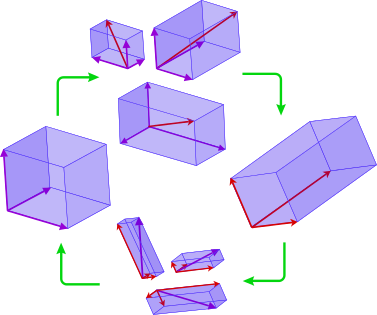
\includegraphics[width=.7\textwidth]{377px-3d_basis_transformation}
\end{figure}

\section*{Keywords}

Change of coordinates matrix, basis representation, trace.

\part{Eigenvectors and Eigenvalues}

\epigraph{\textit{Eigervalves: $E_m(K)$}}{The Big Bang Theory}

\begin{proposition}\label{eigenindependence}
Eigenvectors corresponding to distinct eigenvalues are linearly independent.
\end{proposition}

\begin{proof}
Easy to show for two eigenvectors, then use induction.
\end{proof}

\begin{mdframed}
\begin{theorem}\label{diagonalizable}
A linear operator $T$ on a finite-dimensional vector space $V$ is diagonalizable iff there exists an ordered basis $\beta$ for $V$ consisting of eigenvectors of $T$. Furthermore, if $T$ is diagonalizable, $\beta = \{v_1,\ldots, v_n\}$ is an ordered basis of eigenvectors of $T$, and $D = [T]_\beta$, then $D$ is a diagonal matrix and $D_{jj}$ is the eigenvalue corresponding to $v_j$ for $1 \leq j \leq n$.
\end{theorem}
\end{mdframed}

Proof in the book.

\begin{corollary}
A matrix $A$ is diagonalizable iff the dimensions of its eigenspaces---i.e. the geometric multiplicities over all its eigenvalues---add up to the size of $A$. In this case the geometric multiplicity of each eigenvalue is equal to its algebraic multiplicity.
\end{corollary}

\begin{proof}
By Proposition \ref{eigenindependence}, the eigenspaces are linearly independent. If their dimensions added up to less than $n$, we'd have too few eigenvectors to make a basis for $V$, and by Theorem \ref{diagonalizable}, $A$ would not be diagonalizable. If they added up to more than $n$, we'd have too many linearly independent vectors in $V$. Conversely if they do add up to $n$, then the union of bases for the eigenspaces forms an eigenbasis for $V$, and $A$ is diagonalizable. 
\end{proof}

\begin{proposition}
Let $T$ be a linear operator on a finite-dimensional vector space $V$, and let $\beta$ be an ordered basis for $V$. Then $\lambda$ is an eigenvalue of $T$ iff it is an eigenvalue of $[T]_\beta$.
\end{proposition}

\begin{corollary}
Similar matrices have the same eigenvalues, but not necessarily the same eigenvectors.
\end{corollary}

\begin{proposition}
If $v$ is an eigenvector of $A$ corresponding to eigenvalue $\lambda$, and $B$ is similar to $A$ under change of coordinates matrix $Q$, then $Qv$ is an eigenvector of $B$ corresponding to the same eigenvalue $\lambda$.  Another way of saying this is that change of coordinates preserves eigenvalues and eigenvectors.
\end{proposition}

\begin{proof}
Let $A = Q^{-1}BQ$. Then
\begin{align*}
Av &= Q^{-1}BQv \\
QAv &= BQv \\
\lambda Qv &= BQv,
\end{align*}
so $Qv$ is an eigenvector of $B$ corresponding to $\lambda$.
\end{proof}

\begin{definition}\label{determinantofoperator}
Let $T$ be a linear operator on a finite-dimensional vector space $V$. Define the determinant of $T$ to be $\det T = \det([T]_\beta)$ for any ordered basis $\beta$ for $V$.
\end{definition}

\begin{note}
Since the determinant is multiplicative, for any two bases $\beta$ and $\alpha$ we have
\begin{align*}
\det([T]_\beta) &= \det(Q^{-1} [T]_\alpha Q) \\
&= \det Q^{-1} \det([T]_\alpha) \det Q \\
&= \det([T]_\alpha),
\end{align*}
where $Q = [I]^\alpha_\beta$ is the change of basis matrix from $\beta$ to $\alpha$, and therefore $\det T$ is well defined, i.e. it's independent of the choice of basis.
\end{note}

\begin{proposition}\label{changeofbasislinear}
Representation of a matrix with respect to a basis is a linear operation, i.e. $$[T + \lambda U]_\beta = [T]_\beta + \lambda[U]_\beta.$$ In fact it's an isomorphism. For a fixed basis $\beta$ this transformation is usually written $\Phi_\beta: \mathcal{L}(V) \longrightarrow M_{n\times n}(F).$ See Proposition \ref{matrixbasisrep}.
\end{proposition}

\begin{proof}
Let $v$ be a vector, $\beta = \{v_1,\ldots, v_n\}$, and $T(v) = \sum a_i v_i, U(v) = \sum b_i v_i$. We want to show that
\begin{align*}
[T + \lambda U]_\beta [v]_\beta &= ([T]_\beta + \lambda[U]_\beta)[v]_\beta \\
[T(v) + \lambda U(v)]_\beta &= [T(v)]_\beta + \lambda[U(v)]_\beta.
\end{align*}
The RHS is $[a_i] + \lambda [b_i]$, which is the same as the LHS: $[a_i + \lambda b_i]$.
\end{proof}

\begin{note}
Analogously, the standard representation of a vector space $V$ with respect to a basis $\beta$ is $\phi_\beta: V \longrightarrow F^n.$ And it's also an isomorphism.
\end{note}

\begin{proposition}
For any scalar $\lambda$ and any ordered basis $\beta$ for $V$, $\det(T - \lambda I_V) = \det([T]_\beta - \lambda I)$.
\end{proposition}

\begin{proof}
Follows from Definition \ref{determinantofoperator} and Proposition \ref{changeofbasislinear}.
\end{proof}

\begin{mdframed}
\begin{proposition}[Eigenvalues and invertibility]
A linear operator $T$ on a finite-dimensional vector space is invertible iff its eigenvalues are nonzero.
\end{proposition}
\end{mdframed}

\begin{proof}
If zero is an eigenvalue of $T$, then $\det(T - 0 \cdot I) = 0$, and $T$ is not invertible. Conversely, if $T$ is not invertible, then there exists a nonzero vector $v$ s.t. $T(v) = 0 = 0 \cdot v$, and so 0 is an eigenvalue and $v$ is an eigenvector of $T$.
\end{proof}

\begin{proposition}
Let $T$ be an invertible linear operator. Then a scalar $\lambda$ is an eigenvalue of $T$ iff $\lambda^{-1}$ is an eigenvalue of $T^{-1}$. Note that by the previous proposition $\lambda$ is nonzero, so $\lambda^{-1}$ exists.
\end{proposition}

\begin{proof}
Apply $T^{-1}$ to both sides of $T(v) = \lambda v$.
\end{proof}

\begin{proposition}
The eigenvalues of an upper triangular matrix $M$ are the diagonal entries of $M$.
\end{proposition}

\begin{proof}
Follows from the fact that the determinant of an upper triangular matrix is the product of its diagonal entries.
\end{proof}

\begin{proposition}
Similar matrices have the same characteristic polynomial.
\end{proposition}

\begin{proof}
Let $A = Q^{-1} B Q$. Then 
\begin{align*}
\det(A - tI) &= \det(Q^{-1} B Q - Q^{-1} tI Q) \\
&= \det(Q^{-1}(B - tI)Q) \\
&= \det(Q^{-1})\det(B - tI)\det(Q) \\
&= \det(B - tI).\qedhere
\end{align*}
\end{proof}

\begin{corollary}
The definition of the characteristic polynomial of a linear operator on a finite-dimensional vector space $V$ is independent of the choice of basis for $V$.
\end{corollary}

\begin{proof}
Follows immediately from the fact that similar matrices are the same linear operator expressed under different bases.
\end{proof}

\begin{proposition}
Let $T$ be a linear operator on a finite dimensional vector space $V$ over a field $F$. Let $\beta$ be an ordered basis for $V$, and let $A = [T]_\beta$. Then a vector $v \in V$ is an eigenvector of $T$ corresponding to $\lambda$ iff $\phi_\beta(v)$ is an eigenvector of $A$ corresponding to $\lambda$.
\end{proposition}

\begin{figure}[H]
$$\begin{tikzcd}
V \arrow{r}{T} \arrow[swap]{d}{\phi_\beta} & V \arrow{d}{\phi_\beta} \\
F^n \arrow[swap]{r}{L_A} & F^n
\end{tikzcd}$$
\end{figure}

\begin{proof}
TODO.
\end{proof}

\section{Eigenvectors and Some Special Functions and Matrices}

\begin{lemma}
A square matrix has the same determinant as its transpose.
\end{lemma}

\begin{proposition}
A square matrix has the same characteristic polynomial as its transpose.
\end{proposition}

\begin{proposition}
If $x$ is an eigenvector of $T$ corresponding to $\lambda$, then for any positive integer $m$, $x$ is an eigenvector of $T^m$ corresponding to $\lambda^m$.
\end{proposition}

\begin{proof}
Linearity of $T$ and induction.
\end{proof}

\begin{note}
The same holds for matrices. It's always the same!
\end{note}

\begin{proposition}
Similar matrices have the same trace.
\end{proposition}

\begin{proof}
Follows from Proposition \ref{tracecommutative}.
\end{proof}

\begin{corollary}
Define the trace of a linear operator $T$ on a finite dimensional vector space as $\tr [T]_\beta$ for any basis $\beta$. This is well defined by the previous Proposition.
\end{corollary}

\begin{proposition}
Let $T$ be the linear operator on $M_{n\times n}(\R)$ defined by $T(A) = A^t.$ Then $\pm 1$ are the only eigenvalues of $T.$ The eigenvectors of $T$ corresponding to $\pm 1$ are symmetric and antisymmetric matrices, respectively.
\end{proposition}

\begin{example}
In two dimensions, an ordered basis for $M_{2 \times 2}(\R)$ consisting of eigenvectors of $T$ so that $[T]_\beta$ is a diagonal matrix is 
$$\beta = \left\{ 
\begin{bmatrix}
1 & 0 \\
0 & 0
\end{bmatrix},
\begin{bmatrix}
0 & 0 \\
0 & 1
\end{bmatrix},
\begin{bmatrix}
0 & 1 \\
1 & 0
\end{bmatrix},
\begin{bmatrix}
0 & 1 \\
-1 & 0
\end{bmatrix}
\right\}.$$
The first three matrices are symmetric and correspond to the eigenvalue $+1$, while the last is skew-symmetric and corresponds to $-1.$
\end{example}

\begin{example}
More generally, in $n$ dimensions an eigenbasis consists of symmetric matrices of the form $A$ that has zeroes everywhere except a single $1$ along the diagonal, and symmetric matrices of the form $B$ with zeroes everywhere except a $1$ in two opposite entries $B_{ij}$ and $B_{ji}$, and finally anti-symmetric matrices of the form $C$ with zeroes everywhere except a $-1$ and a $+1$ in two opposite entries $C_{ij}$ and $C_{ji}$, where the $-1$ is in the lower left half and the $+1$ in the upper right half of $C$. There are $n$ matrices of type $A$, $(n^2 - n) / 2$ each of type $B$ and $C$, for a total of $n^2,$ as expected.
\end{example}

\subsection{Scalar Matrices}

\begin{definition}
A scalar matrix is a square matrix of the form $\lambda I$ for some scalar $\lambda$.
\end{definition}

\begin{figure}[H]
\centering
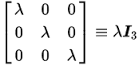
\includegraphics[width=.2\textwidth]{scalarmatrix}
\end{figure}

\begin{proposition}
If a square matrix $A$ is similar to a scalar matrix $\lambda I$, then $A = \lambda I$.
\end{proposition}

\begin{proof}
If $A$ is similar to $\lambda I$, that means there is an invertible matrix $Q$ s.t. $A = Q^{-1} \lambda I Q = \lambda I$.
\end{proof}

\begin{proposition}
A diagonalizable matrix $A$ having only one eigenvalue is a scalar matrix.
\end{proposition}

\begin{proof}
If $A$ is diagonalizable, this means $A$ is similar to a diagonal matrix, whose diagonal entries are its eigenvalues. Since $A$ only has one eigenvalue $\lambda$, the diagonal entries are all equal to $\lambda$.
\end{proof}

\begin{example}
$\begin{bmatrix}
1 & 1 \\
0 & 1 \\
\end{bmatrix}$ is not diagonalizable.
\end{example}

\section*{Keywords}

Eigenvectors, eigenvalues, eigenspace, eigenbasis, differential operator, eigenfunctions, algebraic and geometric multiplicities, scalar matrix, characteristic polynomial, skew / anti-symmetric matrix.

\begin{thebibliography}{99}

\bibitem{FIS} Linear Algebra by Friedberg, Insel, and Spence.

\end{thebibliography}

\end{document}